\documentclass{article}
\usepackage{caption}
\usepackage{amssymb}
\usepackage{array}
\usepackage{geometry}
\usepackage{scrextend}
\usepackage{amsmath}
\usepackage{hyperref}
\usepackage{graphicx}
\usepackage{pdfpages}
\usepackage{multicol}

\title{EE102 Homework 2}
\author{Jacob Guenther}

\geometry{
	a4paper,
	total={170mm,257mm},
	left=20mm,
	top=20mm,
}

\newcommand{\problemstatement}[3]{
\noindent
\begin{tabular}{ m{0.5cm} m{42em} m{0.5cm} }
	({#1}) & {#2} & {#3}pts
\end{tabular}
}

\begin{document}

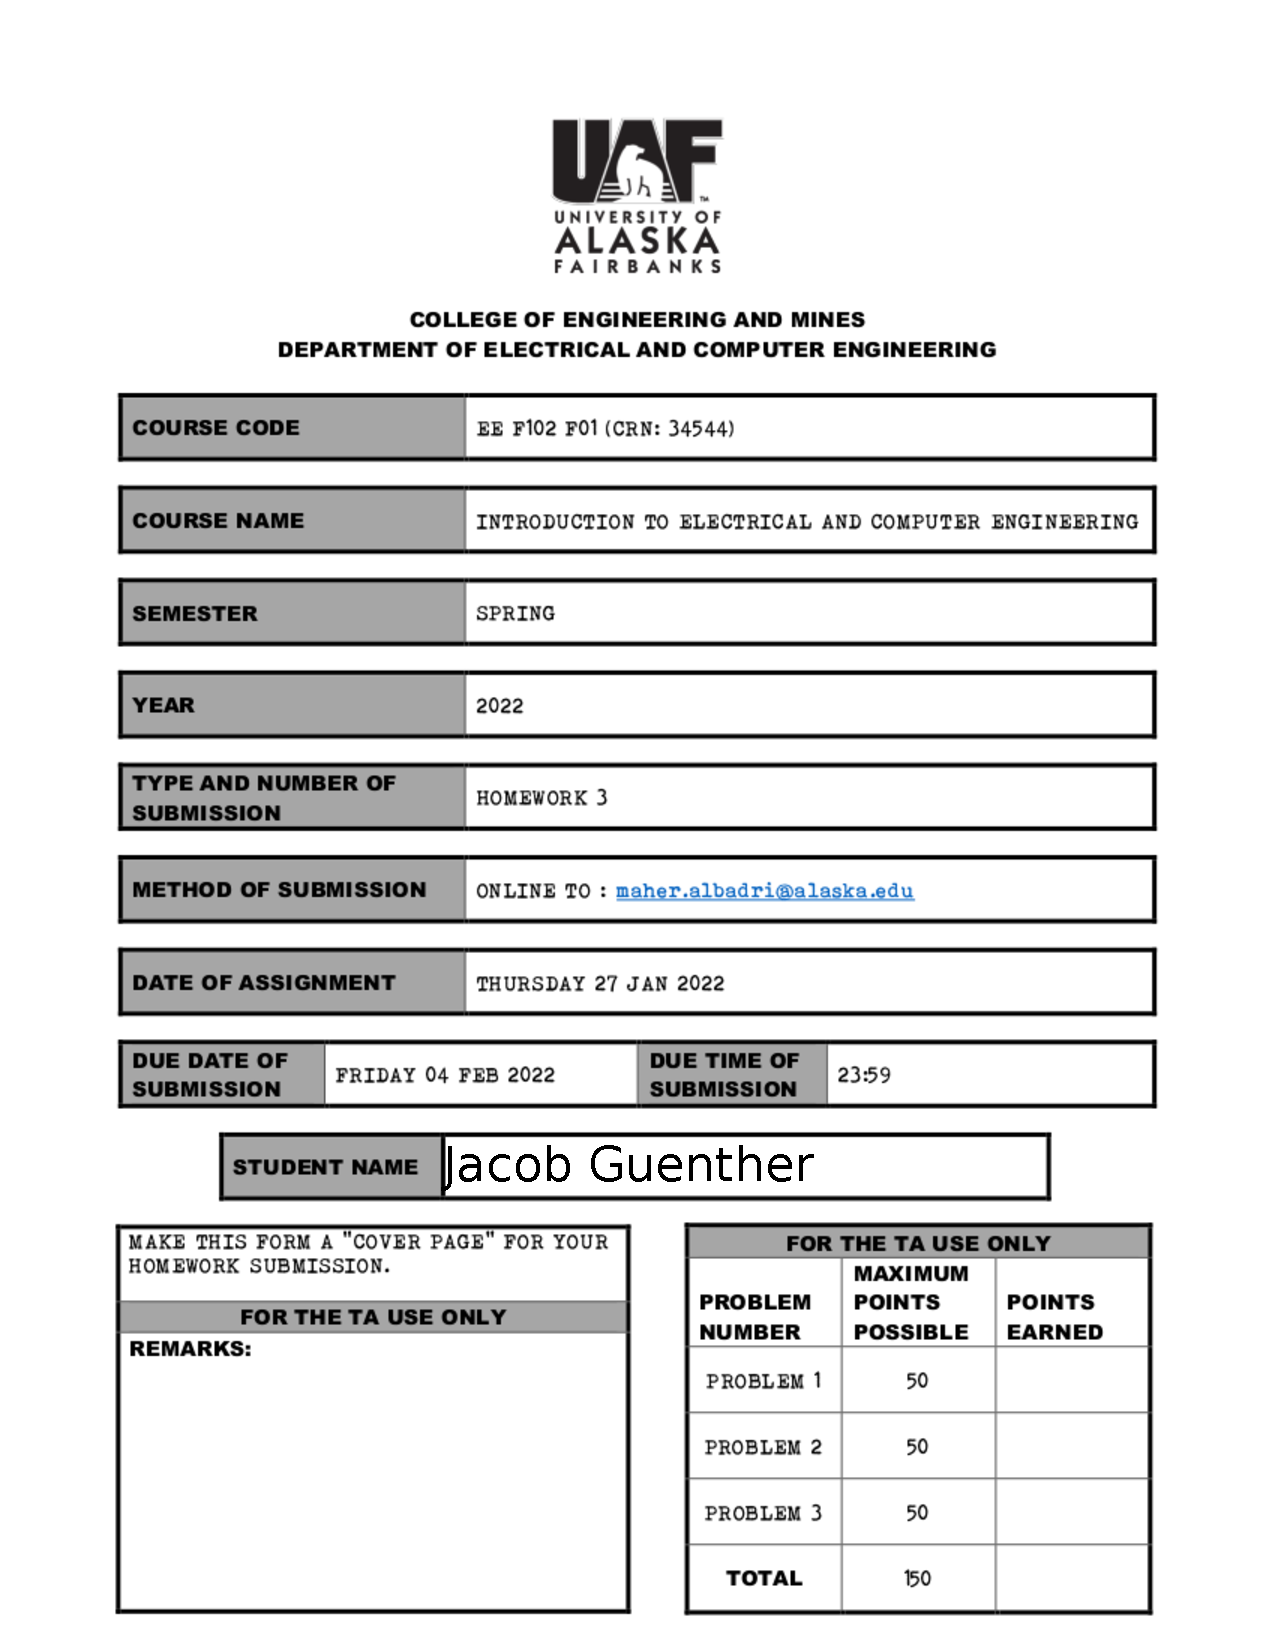
\includepdf[pages=1,pagecommand={}]{HW3_cover.pdf}

\section{Problem HW-3-1}
\problemstatement{1}{For the circuit shown, measurements are conducted and the following data
is made available:}{}
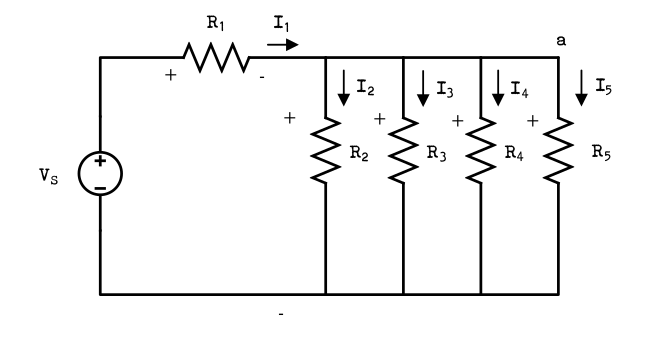
\includegraphics[width=\textwidth]{problem_1_figure}
\begin{itemize}
	\item $\text{V}_\text{s} = 120 \text{V}$
	\item $\text{V}_\text{a} = 73.4 \text{V}$
	\item $\text{P}_\text{s} = 2795 \text{W}$
	\item $\text{P}_\text{1} = 1085 \text{W}$
	\item $\text{P}_\text{2} = 539 \text{W}$
	\item $\text{P}_\text{4} = 385 \text{W}$
	\item $\text{P}_\text{5} = 337 \text{W}$
\end{itemize}
\begin{itemize}
	\item (a) Determine the number of branches. \\
		There are \textbf{6 branches} in the circuit. 5 resistors and 1 voltage source.
	\item (b) Determine the number of nodes. \\
		There are \textbf{3 nodes} in the circuit.
		\begin{itemize}
			\item between $\text{V}_\text{s}$ and $\text{R}_\text{1}$
			\item between $\text{R}_\text{1}$, $\text{R}_\text{2}$, $\text{R}_\text{3}$, $\text{R}_\text{4}$, and $\text{R}_\text{5}$
			\item between $\text{R}_\text{2}$, $\text{R}_\text{3}$, $\text{R}_\text{4}$, $\text{R}_\text{5}$, and $\text{V}_\text{s}$
		\end{itemize}
	\item (c) Determine the number of independent loops. \\
		\textbf{Note:}
		\begin{equation}
			l = b - n + 1
		\end{equation}
		\textbf{Solution:}
		\begin{align*}
			\text{let } b &= 6 \\
			\text{let } n &= 3 \\
			l &= 6 - 3 + 1 \\
			&= 4 \text{ independent loops}
		\end{align*}
		\textbf{Answer:} There are \textbf{4 independent loops} in the circuit.
	\item (d) Determine $\text{P}_3$. \\
		\textbf{Note:}
		\begin{equation}
			\sum{P_i} = 0
		\end{equation}
		\textbf{Solution}
		\begin{align*}
			2795 \text{W} &= 539 \text{W} + \text{P}_3 + 385 \text{W} + 337 \text{W} \\
			\text{P}_3 &= 1261 \text{W} - 2795 \text{W} \\
			&= 1534 \text{W}
		\end{align*}
		\textbf{Answer:} \textbf{$\text{P}_3$ = 1534 W}
	\item (e) Determine $\text{I}_1$. \\
		\textbf{Note:}
		\begin{equation}
			(closed loop) \sum{\text{V}_i} = 0
		\end{equation}
		\begin{equation}
			\text{P} = \text{I} \cdot \text{V}
		\end{equation}
		\textbf{Solution:}
		\begin{align*}
				\text{V}_1 &= \text{V}_s - \text{V}_a \\
				&= 120 \text{V} - 73.4 \text{V} \\
				&= 46.6 \text{V} \\
				\text{I}_1 &= {1084 \text{W} \over 46.6 \text{V}} \\
				&= 23.26 \text{A}
		\end{align*}
		\textbf{Answer:} \textbf{$\text{I}_1$ = 23.26 A}
	\item (f) Determine $\text{I}_3$. \\
		\textbf{Solution:}
		\begin{align*}
			\text{I}_3 &= { \text{P}_3 \over \text{V}_a } \\
			&= { 1534 \text{W} \over 73.4 \text{V} } \\
			&= 20.9 \text{A} \\
		\end{align*}
		\textbf{Answer:} \textbf{$\text{I}_3$ = 20.9 A}
\end{itemize}

\newpage
\section{Problem HW-3-2}
\problemstatement{1}{For the circuit shown, measurements are conducted and the following data
is made available:}{}
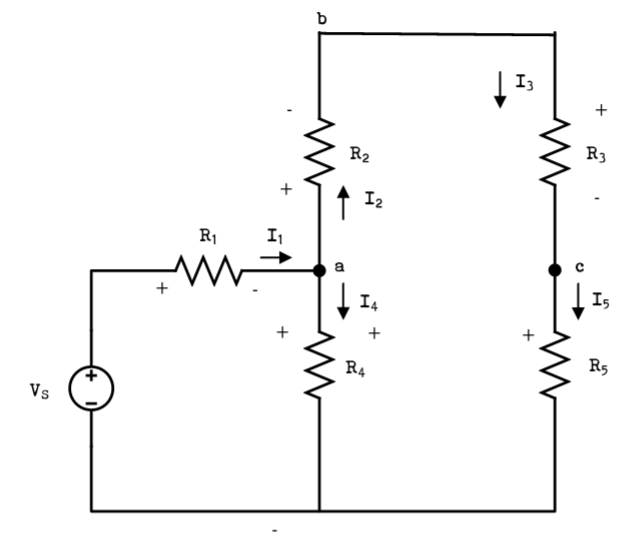
\includegraphics[width=\textwidth]{problem_2_figure}
\begin{itemize}
	\item $\text{V}_\text{s} = 120 \text{V}$
	\item $\text{V}_\text{a} = 72 \text{V}$
	\item $\text{V}_\text{b} = 48 \text{V}$
	\item $\text{V}_\text{c} = 24 \text{V}$
	\item $\text{P}_\text{s} = 1152 \text{W}$
	\item $\text{P}_\text{1} = 460.8 \text{W}$
	\item $\text{I}_\text{4} = 7.2 \text{A}$
\end{itemize}
\begin{itemize}
	\item (a) Determine the number of branches. \\
		There are \textbf{6 branches} in the circuit. 5 resistors and 1 voltage source.
	\item (b) Determine the number of nodes. \\
		There are \textbf{5 nodes} in the circuit.
		\begin{itemize}
			\item between $\text{V}_\text{s}$ and $\text{R}_\text{1}$
			\item between $\text{R}_\text{1}$, $\text{R}_\text{2}$, and $\text{R}_\text{4}$
			\item between $\text{R}_\text{2}$, and $\text{R}_\text{3}$
			\item between $\text{R}_\text{3}$, and $\text{R}_\text{4}$
			\item between $\text{V}_\text{s}$, $\text{R}_\text{4}$, and $\text{R}_\text{5}$
		\end{itemize}
	\item (c) Determine the number of independent loops.\\
		\textbf{Solution:}
		\begin{align*}
			\text{let } b &= 6 \\
			\text{let } n &= 5 \\
			l &= 6 - 5 + 1 \\
			&= 2 \text{ independent loops}
		\end{align*}
		\textbf{Answer:} There are \textbf{2 independent loops} in the circuit.
		\item (d) Determine $\text{V}_{ac}$.
		\textbf{Note:}
		\begin{align*}
			\text{Note } \text{V}_a = 72 \text{V} \\
			\text{Note } \text{V}_c = 24 \text{V} \\
		\end{align*}
		\begin{align*}
			\text{V}_{ac} &= \text{V}_a - \text{V}_c \\
			&= 72 \text{V} - 24 \text{V} \\
			&= 48 \text{V}
		\end{align*}
		\textbf{Answer:} \textbf{$\text{V}_{ac}$ = 48 V}
	\item (e) Determine $\text{P}_2$. \\
		\textbf{Note:}
		\begin{equation}
			\sum{I_{in}} = \sum{I_{out}}
		\end{equation}
		\textbf{Solution:} \\
		\begin{align*}
			\text{V}_1 &= 120 \text{V} - 72 \text{V} \\
			&= 48 \text{V} \\
			\text{I}_1 &= { \text{P}_1 \over \text{V}_1 } \\
			&= { 460.8 \text{W} \over 48 \text{V} } \\
			&= 9.6 \text{A} \\
			\text{I}_1 &= \text{I}_2 + \text{I}_4 \\
			\text{I}_2 &= 9.6 \text{A} - 7.2 \text{A} \\
			&= 2.4 \text{A} \\		
			\text{V}_2 &= \text{V}_{ab} \\
			&= \text{V}_a - \text{V}_b \\
			&= 72 \text{V} - 48 \text{V} \\
			&= 24 \text{V} \\
			\text{P}_2 &= \text{I}_2 * \text{V}_2 \\
			&= 2.4 \text{A} \cdot 24 \text{V} \\
			&= 57.6 \text{W}
		\end{align*}
		\textbf{Answer:} \textbf{$\text{P}_{2}$ = 57.6 W}
	\item (f) Determine $\text{P}_3$. \\
		\textbf{Note:}
		\begin{align*}
			\text{V}_\text{b} &= 48 \text{V} \\
			\text{V}_\text{c} &= 24 \text{V} \\
			\text{I}_2 &= 2.4 \text{A} \\
		\end{align*}
		\textbf{Solution:}
		\begin{align*}
			\text{I}_2 &= \text{I}_3 \\
			\text{I}_3 &= 2.4 \text{A} \\
			\text{V}_{bc} &= \text{V}_{b} - \text{V}_{c} \\
			&= 48 \text{V} - 24 \text{V} \\
			&= 24 \text{V} \\
			\text{P}_3 &= \text{I}_3 \cdot \text{V}_{ab} \\
			&= 2.4 \text{A} \cdot 24 \text{V} \\
			&= 57.6 \text{W}
		\end{align*}
		\textbf{Answer:} \textbf{$\text{P}_{3}$ = 57.6 W}
	\item (g) Determine $\text{P}_4$. \\
		\textbf{Note:}
		\begin{align*}
			\text{V}_\text{a} &= 72 \text{V} \\
			\text{I}_4 &= 7.2 \text{A} \\
		\end{align*}
		\textbf{Solution:}
		\begin{align*}
			\text{P}_4 &= \text{I}_4 \cdot \text{V}_a \\
			&= 7.2 \text{A} \cdot 72 \text{V} \\
			&= 518.4 \text{W}
		\end{align*}
		\textbf{Answer:} \textbf{$\text{P}_{4}$ = 518.4 W}
	\item (h) Determine $\text{P}_5$. \\
		\textbf{Note:}
		\begin{align*}
			\text{V}_\text{c} &= 24 \text{V} \\
			\text{I}_2 &= 2.4 \text{A} \\
		\end{align*}
		\textbf{Solution:}
		\begin{align*}
			\text{I}_2 &= \text{I}_3 = \text{I}_5 = 2.4 \text{A} \\
			\text{P}_5 &= \text{I}_5 \cdot \text{V}_c \\
			&= 2.4 \text{A} \cdot 24 \text{V} \\
			&= 57.6 \text{W}
		\end{align*}
		\textbf{Answer:} \textbf{$\text{P}_{4}$ = 57.6 W}
\end{itemize}

\newpage
\section{Problem HW-3-1}
\problemstatement{1}{For the circuit shown, measurements are conducted and the following data
is made available:}{}
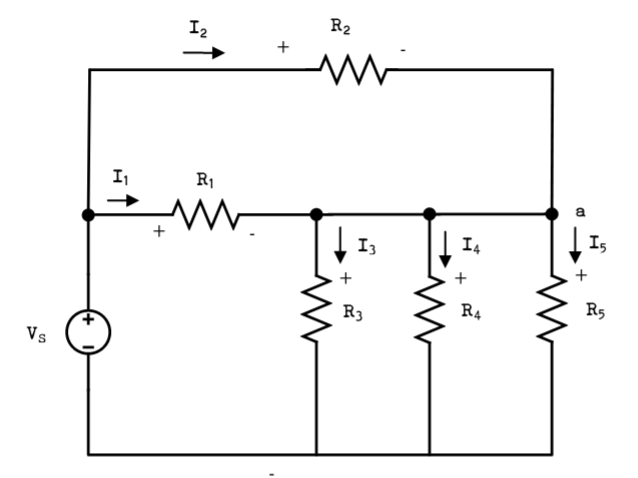
\includegraphics[width=\textwidth]{problem_3_figure}
\begin{itemize}
	\item $\text{V}_\text{s} = 120 \text{V}$
	\item $\text{V}_\text{a} = 48 \text{V}$
	\item $\text{P}_\text{s} = 1728 \text{W}$
	\item $\text{P}_\text{1} = 518.4 \text{W}$
	\item $\text{P}_\text{3} = \text{P}_\text{4} = \text{P}_\text{5} = 230.4 \text{W}$
\end{itemize}
\begin{itemize}
	\item (a) Determine the number of branches. \\
	There are \textbf{6 branches} in the circuit. 5 resistors and 1 voltage source.
	\item (b) Determine the number of nodes. \\
		There are \textbf{3 nodes} in the circuit.
		\begin{itemize}
			\item between $\text{V}_\text{s}$, $\text{R}_\text{1}$, and $\text{R}_\text{2}$
			\item between $\text{R}_\text{1}$, $\text{R}_\text{2}$, $\text{R}_\text{3}$, $\text{R}_\text{4}$, and $\text{R}_\text{5}$
			\item between $\text{V}_\text{s}$, $\text{R}_\text{3}$, $\text{R}_\text{4}$, and $\text{R}_\text{5}$
		\end{itemize}
	\item (c) Determine the number of independent loops.
		\begin{align*}
			\text{let } b &= 6 \\
			\text{let } n &= 3 \\
			l &= 6 - 3 + 1 \\
			&= 4 \text{ independent loops}
		\end{align*}
		\textbf{Answer:} There are \textbf{4 independent loops} in the circuit.
	\item (d) Determine $\text{P}_2$. \\
		\textbf{Solution:}
		\begin{align*}
			\sum{P_i} &= 0 \\
			0 &= \text{P}_s + \text{P}_1 + \text{P}_2 + \text{P}_3 + \text{P}_4 + \text{P}_5 \\
			 \text{P}_2 &= -\text{P}_s - \text{P}_1 - \text{P}_3 - \text{P}_4 - \text{P}_5 \\
			&= 1728  \text{W} - 518.4 \text{W} - 230.4 \text{W} - 230.4 \text{W} - 230.4 \text{W} \\
			&= 518.4 \text{W}
		\end{align*}
		\textbf{Answer:} \textbf{$\text{P}_{2}$ = 518.4 W}
	\item (e) Determine $\text{I}_3$.
	\item (f) Determine $\text{I}_4$.
	\item (g) Determine $\text{I}_5$. \\
		\textbf{Note:}
		\begin{align*}
			\text{V}_a &= 48 \text{V} \\
			\text{P}_3 = \text{P}_4 = \text{P}_5 &= 230.4 \text{W}
		\end{align*}
		\textbf{Solution:}
		\begin{align*}
			\text{I}_3 &= { \text{P}_3 \over \text{V}_a } \\
			&= { 230.4 \text{W} \over 48 \text{V} } \\
			&= 4.8 \text{A} \\
			\text{I}_3 = \text{I}_4 = \text{I}_5 &= 4.8 \text{A}
		\end{align*}
		\textbf{Answer:}
		\begin{itemize}
			\item[(e)] \textbf{$\text{I}_{3}$ = 4.8 A}
			\item[(f)] \textbf{$\text{I}_{4}$ = 4.8 A}
			\item[(g)] \textbf{$\text{I}_{5}$ = 4.8 A}
		\end{itemize}
\end{itemize}

\newpage
\section{References}
[1] Denise Thorsen, Maher Al-Badri, INTRODUCTION TO ELECTRICAL AND COMPUTER ENGINEERING, University of Alaska Fairbanks, 2022.

\end{document}